%{{{ Formatierung

\documentclass[a4paper,12pt]{article}

\usepackage{physics_notetaking}

%%% dark red
%\definecolor{bg}{RGB}{60,47,47}
%\definecolor{fg}{RGB}{255,244,230}
%%% space grey
%\definecolor{bg}{RGB}{46,52,64}
%\definecolor{fg}{RGB}{216,222,233}
%%% purple
%\definecolor{bg}{RGB}{69,0,128}
%\definecolor{fg}{RGB}{237,237,222}
%\pagecolor{bg}
%\color{fg}

\newcommand{\td}{\,\text{d}}
\newcommand{\RN}[1]{\uppercase\expandafter{\romannumeral#1}}
\newcommand{\zz}{\mathrm{Z\kern-.3em\raise-0.5ex\hbox{Z} }}

\newcommand\inlineeqno{\stepcounter{equation}\ {(\theequation)}}
\newcommand\inlineeqnoa{(\theequation.\text{a})}
\newcommand\inlineeqnob{(\theequation.\text{b})}
\newcommand\inlineeqnoc{(\theequation.\text{c})}

\newcommand\inlineeqnowo{\stepcounter{equation}\ {(\theequation)}}
\newcommand\inlineeqnowoa{\theequation.\text{a}}
\newcommand\inlineeqnowob{\theequation.\text{b}}
\newcommand\inlineeqnowoc{\theequation.\text{c}}

\renewcommand{\refname}{Source}
\renewcommand{\sfdefault}{phv}
%\renewcommand*\contentsname{Contents}

\pagestyle{fancy}

\sloppy

\numberwithin{equation}{section}

%}}}

\begin{document}

%{{{ Titelseite

\title{Übersichtsprüfung Experimentalphysik 1 bis 3}
\author{Jonas Wortmann}
\maketitle
\pagenumbering{gobble}

%}}}

\newpage

%{{{ Inhaltsverzeichnis

\fancyhead[L]{\thepage}
\fancyfoot[C]{}
\pagenumbering{arabic}

\tableofcontents

%}}}

\newpage

%{{{

\fancyhead[R]{\leftmark\\\rightmark}

\newpage
\section{Mechanik}
\subsection{Schiefer Wurf}
Die Bewegungsgleichung des schiefen Wurfs ist gegeben durch
\begin{align} 
        \vv{x}\left(t\right)&=\begin{pmatrix}
                x\left(t\right)\\y\left(t\right)
        \end{pmatrix}\\
                            &=\begin{pmatrix}
                                    v_0\cos \left(\varphi \right)t\\
                                    -\tfrac{1}{2}gt^2+v_0\sin \left(\varphi \right)t+y_0
                            \end{pmatrix}
.\end{align} 
Die $y$--Richtung berechnet sich aus der Integration der Geschwindigkeit
\begin{align} 
        y\left(t\right)&=\int_{0}^{t}\td tv_y\left(t\right)=\int_{0}^{t}\td t\left(v_0-gt\right)
.\end{align} 

\subsection{\textsc{Newton}'sche Kraftgesetze}
1. Ein kräftefreier Körper bleibt im Zustand der Ruhe, wenn er vorher in Ruhe war bzw.\ in gleichförmiger Bewegung, wenn er vorher in gleichförmiger Bewegung war. (Ein Intertialsystem ist ein Bezugssystem, in dem diese Gesetzmäßigkeit gilt)\par\noindent
2. Die Kraft ist gegeben durch $\vv{F}=m\vv{a}$.\par\noindent
3. Übt ein Körper 1 eine Kraft auf einen Körper 2 aus, so übt der Körper 2 eine gleichgroße entgegengerichtete Kraft auf Körper 1 aus.

\subsection{\textsc{Kepler}'schen Gesetze}
1. Alle Planeten kreisen auf elliptischen Bahnen um ihr Zentralgestirn. 
Das Baryzentrum des Systems liegt in einem der Brennpunkte.\\
2. Der Fadenstrahl der Planeten überstreicht in gleichen Zeiten gleiche Flächen.
Es gilt
\begin{align} 
        \vv{L}&=\vv{r}\times \vv{p}=m\left(\vv{r}\times \vv{v}\right)=\text{const.}
.\end{align} 
Betrachtet man die Änderung der Fläche über die Zeit, gilt
\begin{align} 
        \td A&=\dfrac{1}{2}\left(\vv{r}\times \td\vv{r}\right)\\
        \diff[]{A}{t}&=\dfrac{1}{2}\left(\vv{r}\times \vv{v}\right)
.\end{align} 
Daraus folgt, dass
\begin{align} 
        \diff[]{A}{t}=\dfrac{1}{2}\dfrac{\vv{L}}{m}=\text{const.}
.\end{align}
3. Die Quadrate der Umlaufzeiten der Planeten sind proportional zu den Kuben der großen Halbachse.

\subsection{\textsc{Galilei}--Transformation}
Die \textsc{Galilei}--Transformation transformiert ein Bezugssystem $\Sigma$ in ein anderes Bezugssystem $\Sigma'$, welches sich mit einer konstanten Geschwindigkeit relativ zu $\Sigma$ bewegt.
\begin{align} 
        \vv{r}'&=\vv{r}-\vv{v}t\\
        t'&=t
.\end{align} 
Längen und Beschleunigung sind \textsc{Galilei}--invariant; die Geschwindigkeit selbst nicht.\par
Die Transformation in das Schwerpunktsystem sieht wie folgt aus
\begin{align} 
        R&=\dfrac{m_ir_i}{M}\\
        r^*_i&=r_i-R\\
        v^*_i&=v_i-v
.\end{align} 
$v$ bezeichnet hier die Geschwindigkeit des Schwerpunktes gegenüber dem Intertialsystem.

\subsection{Beschleunigte und rotierende Bezugssysteme; Scheinkräfte}
Scheinkräfte treten in beschleunigten und rotierenden Bezugssystemen auf, da der Bezugspunkt des Systems auch beschleunigt wird.
Die \textsc{Galilei}--Trafo ist hier nicht mehr anzuwenden, da die Geschwindigkeit nicht konstant ist.
\begin{align} 
        \vv{r}'&=\vv{r}-\vv{v}t\\
        \ddot{\vv{r}}'&=\ddot{\vv{r}}-\dot{\vv{v}}
.\end{align} 
Aus dieser Beschleunigung ergibt sich die Scheinkraft im beschleunigten Bezugssystem.
Wichtig sind folgende Kräfte
\begin{align} 
        \vv{F}_\text{Coriolis}&=2m\left(\vv{v}\times \vv{\omega }\right)\\
        \vv{F}_\text{Zentrifugal}&=m\vv{\omega }\times \left(\vv{r}\times \vv{\omega }\right)
.\end{align} 

\subsection{Raketengleichung}
Die Rakete ist ein System mit veränderlicher Masse.
Die wirkende Kraft ist also abhängig von der Änderung der Masse.
Zum Zeitpunkt $t$ fliegt die Rakete mit einem Impuls von $\vv{p}=m\vv{v}$. 
Verliert die Rakete durch den Antrieb Masse, so ändert sich der Impuls zu
\begin{align} 
        \vv{p}_{+\td t}&=\left(m+\td m\right)\left(\vv{v}+\vv{\td v}\right)+\left(-\td m\right)\left(\vv{v}-\vv{v}_\text{Gas}\right)\\
              &=m\vv{v}+m\vv{\td v}+\td m\vv{v}+\td m\vv{\td v}-\td m \vv{v}+\td m \vv{v}_\text{Gas}\\
              &=m\vv{v}+m\vv{\td v}+\td m \vv{v}_\text{Gas}+\underbrace{\td m\vv{\td v}}_{\approx 0}
.\end{align} 
Da der Gesamtimpuls erhalten ist, gilt $\vv{p}_{+\td t}=\vv{p}=m\vv{v}$, also
\begin{align} 
        m\vv{v}&=m\vv{v}+m\vv{\td v}+\td m \vv{v}_\text{Gas}\\
        \int_{v_0}^{v\left(t\right)}\vv{\td v}&=-\vv{v}_\text{Gas}\int_{m_0}^{m\left(t\right)}\td m\dfrac{1}{m}\\
        \vv{v}\left(t\right)-\vv{v}_0&=-\vv{v}_\text{Gas}\ln\left(\dfrac{m\left(t\right)}{m_0}\right)
.\end{align} 

\subsection{\textsc{Foucault}--Pendel}
Das \textsc{Foucault}--Pendel ist ein Pendel, dessen Schwingebene durch die Corioliskraft gedreht wird.
Dadurch kann die Rotationsbewegung der Erde nachgewiesen werden.
Die Corioliskraft ist eine Trägheitskraft, die in einem rotierendem Bezugssystem auftritt.
Sie tritt auf, wenn sich ein Körper nicht parallel zur Rotationsachse bewegt.
\begin{align} 
        \vv{F}_C=2m\vv{v}\times \vv{\omega }
.\end{align} 
Da die Kraft senkrecht zur Geschwindigkeit ist, bewirkt sie nur eine Ablenkung zur Seite und keine Vergrößerung oder Verkleinerung der Geschwindigkeit.\par
Der Zusammenhang mit dem \textsc{Foucault}--Pendel besteht darin, dass das Pendel bei der Pendelbewegung zur Seite abgelenkt wird und so seine Pendeleben dreht. 
An den Polen (also liegt der Aufhängepunkt des Pendels in der Rotationsachse) rotiert das Pendel genau entgegengesetzt zur Erde.
Eine vollständige Rotation der Pendelebene ist nach einer vollständigen Rotation der Erde.\par
Am Äquator rotiert die Pendelebene gar nicht.

\subsection{Konservative Kräfte}
Eine Kraft ist konservativ, wenn gilt
\begin{enumerate}[label=--]
        \item Das Kraftfeld ist nicht zeitabhängig.
        \item Das Kraftfeld ist wirbelfrei. $\vv{\text{rot}}\vv{F}\left(\vv{r}\right)=\vv{0}$.
        \item Die Arbeit über alle geschlossenen Kurven ist null. Die Arbeit über eine nicht geschlossene Kurve ist nur von ihrem Anfangs-- und Endpunkt abhängig. $\,\forall \mathcal{C}:\oint_{C}^{}\td \vv{r}\vv{F}\left(\vv{r}\right)=0$.
        \item Das Kraftfeld ist das Gradientenfeld eines Potentials. $\vv{F}\left(\vv{r}\right)=-\vv{\text{grad}}V\left(r\right)$.
\end{enumerate}

\subsection{Stöße}
Bei einem elastischen Stroß gilt die Impuls-- und Energieerhaltung
\begin{align} 
        \vv{p}_1+\vv{p}_2&=\vv{p}_1'+\vv{p}_2'\\
        E_1+E_2&=E_1'+E_2'
.\end{align} 
Bei einem inelastischen Stoß gilt die Impulserhaltung, allerdings nicht die Energieerhaltung, da Energie in Verformung oder Wärme verloren geht
\begin{align} 
        \vv{p}_1+\vv{p}_2&=\vv{p}_1'+\vv{p}_2'\\
        E_1+E_2&=E_1'+E_2'-Q
.\end{align} 
$Q$ beschreibt hier die Menge an Energie die verloren geht.\par
Der Gesamtimpuls im Schwerpunktsystem ist null, da die einzelnen Impulse entgegengerichtet sind,
\begin{align} 
        \vv{p}_1+\vv{p}_2&=0=\vv{p}_1'+\vv{p}_2'
.\end{align} 

\subsection{Experimentelle Bestimmung der Gravitationskonstante}
Die experimentelle Bestimmung der Gravitationskonstante erfolgt über die Gravitationswaage. 
Die Gravitationswaage ist aus einem Torsionsdraht aufgebaut, an dem eine Hantel hängt.
Die Hantel wird von zwei Massen aufgrund der Gravitationskraft ausgelenkt.
Mit der Rückstellkraft des Torsionsdrahtes stellt sich dann ein Gleichgewicht ein
\begin{align} 
        F_r&=2F_\gamma \\
        k\varphi &=2\gamma \dfrac{m_1m_2}{r_{12}^2}\\
        \gamma &=\dfrac{k\varphi r_{12}^2}{2m_1m_2}
.\end{align} 
Hier ist die Gravitationskraft gleich $2F_\gamma $, da zwei Kugeln verwendet werden, um das Pendel auszulenken.

\subsection{Fluchtgeschwindigkeit}
Die Fluchtgeschwindigkeit eines Gravitationspotentials ist erreicht, wenn die kinetische Energie gleich der potentiellen Energie des Potentials ist
\begin{align} 
        \dfrac{1}{2}mv^2&=\dfrac{GMm}{r}\\
        v&=\,\sqrt[]{\dfrac{2GM}{r}}
.\end{align} 
Existieren mehrere Gravitationspotentiale ist die potentielle Energie die Superposition dieser Potentiale (mit korrespondierendem Abstand $r$).\\\indent
Damit ein Körper auf einer elliptischen Bahn um einen anderen Körper kreist, muss die Zentripetalkraft gleich der Gravitationskraft sein
\begin{align} 
        m\dfrac{v^2}{r}&=\dfrac{GM}{r^2}\\
        v&=\,\sqrt[]{\dfrac{GM}{r}}
.\end{align} 

\subsection{Trägheitstensor}
Das Trägheitsmoment gibt die Trägheit eines Körpers bei der Rotation an.
Die Einträge in den Trägheitstensor sind definiert als
\begin{align} 
        I_{ij}&=\rho \int_{V}^{}\td V\left[|\vv{r}|^2\delta _{ij}-r_ir_j\right]
.\end{align} 
Der Satz von \textsc{Steiner} besagt, dass das zusätzliche Trägheitsmoment, welches durch die Verschiebung der Rotationsachse hinzukommt, addiert werden kann, falls die neue Rotationsachse parallel zur vorherigen Rotationsachse ist.
Mit der Distanz $a$, um die verschoben wurde, gilt dann
\begin{align} 
        I=I'+ma^2
.\end{align} 

\subsection{Kreisel}
Die Hauptträgheitsachsen sind die Achsen eines Körpers auf denen dieser Körper den korrespondierenden Eigenwert als Trägheitsmoment hat.\\\indent
Ist $I_1<I_2=I_3$, ist der Körper ein Prolat. 
Ist $I_1=I_2<I_3$, ist der Körper ein Oblat.
Ist $I_1=I_2=I_3$, ist der Körper sphärisch.\\\indent
Ein Kreisel ist symmetrisch, wenn dieser zwei gleiche Hauptträgheitsmomente hat.
Ist dieser Körper auch rotationssymmetrisch und diese Achse, so heißt sie Figurenachse.\\\indent
Präzession beschreibt die Rotation des Drehimpulsvektors eines rotierenden Körpers um eine feste Raumachse.
Diese Rotation tritt auf, wenn ein Drehmoment orthogonal zum Drehimpuls wirkt.
Da die Kraft orthogonal wirkt, wird nur die Richtung des Drehimpulses und nicht seine Länge verändert.\\\indent
Nutation beschreibt die Schwingung des Drehimpulsvektors um die Figurenachse, hervorgerufen durch ein Drehmoment weiteres orthogonales Drehmoment.

\externaldocument{main}
\newpage
\section{Thermodynamik}
\subsection{Temperaturskala (Kelvin)}
Die Fixpunkte der Kelvinskala liegen bei
\begin{enumerate}[label=--]
        \item $\SI{0}{K}$: Absoluter Nullpunkt; das System ist enthält keine kinetische Energie mehr.
        \item $\SI{273,16}{K}\,\text{und}\,\SI{613}{Pa}$: Tripelpunkt von Wasser (\ref{fig:phasendiagramme}), der Zustand bei dem alle Phasen von Wasser miteinander im Gleichgewicht stehen.
\end{enumerate}
Der Tripelpunkt ist in dem Phasendiagramm dargestellt, welches eine gängige Methode ist, die Phase eines Stoffes oder Systems mit Hilfe des Drucks und der Temperatur darzustellen.

\subsection{Wärmeausdehnung von Festkörpern}
Stoffe dehnen sich bei Wärmezufuhr aus, da das \textsc{Lennard}--\textsc{Jones}--Potential eine asymmetrische Form hat. 
Wird Energie in Form von Wärme zu einem Stoff hinzugefügt, erhöht sich die kinetische Energie der Moleküle und so auch die Schwingungsampiltude.
Da das \textsc{Lennard}--\textsc{Jones}--Potential asymmetrisch ist, erhöht sich der mittlere Abstand zwischen den Molekülen.\\\indent
Bei genügend Wärme findet ein Phasenübergang statt.
Da die Form des \textsc{Lennard}--\textsc{Jones}--Potential eine Material-- bzw.\ Stoffeigenschaft ist, haben unterschiedliche Materialien unterschiedlich starke Ausdehnung.\\\indent
Die Länge des Materials nach der Ausdehnung ist gegeben als 
\begin{align} 
        l&=l_0+l_0\alpha _V\Delta T=l_0\left(1+\alpha _l\Delta T\right)&\dfrac{\alpha _l^a}{\alpha _l^b}&=\text{const.}
.\end{align} 
Analog gilt für das Volumen (auch das Gesetz von \textsc{Gay--Lussac})
\begin{align} 
        V&=V_0+V_0\alpha _V\Delta T=V_0\left(1+\alpha _V\Delta T\right)&\dfrac{\alpha _V^a}{\alpha _V^b}&=\text{const.}
.\end{align} 
Für ideale Gase gilt sogar
\begin{align} 
        \dfrac{\alpha _V^a}{\alpha _V^b}=1
.\end{align} 

\subsection{Ideale Gase / \textsc{Van--der--Waals}--Gase}
Ein ideales Gas besteht aus ausdehnungslosen Massenpunkten, belegen also in ihrem Raum kein Volumen.
Zudem sind die Teilchen frei und üben keine Wechselwirkung aufeinander aus.
Ideale Gasteilchen rotieren bzw.\ vibrieren nicht; die Energie ist ausschließlich durch ihre kinetische Energie gegeben.
Ein reales Gas ist näherungsweise ein ideales Gas, wenn es sich weit von seinen Phasenübergängen befindet.\\\\
Das Gesetz von \textsc{Gay--Lussac} besagt
\begin{align} 
        V\left(p_0,\Delta T\right)=V\left(p_0,\Delta T\right)\left(1+\alpha \Delta T\right)
.\end{align} 
Das Gesetz von \textsc{Boyle--Mariotte} besagt
\begin{align} 
        pV\left(p,\Delta T\right)&=p_0V\left(p_0,\Delta T\right)
.\end{align} 
Es folgt also das \textsc{Boyle--Mariotte--Gay--Lussac} Gesetz
\begin{align} 
        pV&=p_0V\left(p_0,\Delta T\right)=p_0V_0\left(1+\alpha \Delta T\right)
.\end{align} 
Für ideale Gase ist $\alpha =\left(\SI{273,15}{\celsius}\right)^{-1}$ bei einer Temperatur von $T=\SI{0}{\celsius}$.\\\indent
Es foglt das ideale Gasgesetz für ein System aus $n$ mol Teilchen
\begin{align} 
        pV&=nRT&R&=\dfrac{p_NV_M}{T_{>0}}
,\end{align} 
mit $V_M$ dem Molvolumen und $p_N$ dem Normaldruck.\\\indent
Für ein reales Gas gilt allerdings näherungsweise
\begin{align} 
        \left(p+\dfrac{an^2}{V^2}\right)\left(V-b\right)&=nRT
,\end{align} 
mit $a$ dem Binnendruck, hervorgerufen durch den Druck der einzelnen Moleküle, und $b$ dem Kovolumen, dem Eigenvolumen der Moleküle.

\subsection{Wärme}
Wärme ist der Teil der Energie, der von einem thermodynamischen System aufgenommen oder abgegeben wird.
Es gibt verschiedene Arten des Wärmeaustausch.
\begin{enumerate}[label=--]
        \item Wärmestrahlung: Wärme wird in der Form von elektromagnetischen Wellen aufgrund von Molekülschwingungen abgestrahlt.
        \item Konduktion: Wärme wird an der Grenze zwischen zwei Oberflächen in Richtung der kälteren Oberfläche abgegeben.
        \item Konvektion: Wärme wird von einem kälteren strömenden Material aufgenommen, indem dieses durch seinen Bewegung immer wieder mit seiner kalten Oberfläche Wärme abtransportieren kann.
\end{enumerate}

\subsection{\textsc{Maxwell}--\textsc{Boltzmann}--Verteilung}
Die \textsc{Maxwell--Boltzmann}--Verteilung beschreibt die statistische Geschwindigkeitsverteilung eines idealen Gases. 
Wichtig dabei ist, dass die Verteilung eine lang auslaufende Kurve besitzt.
Es können also Gasmoleküle existieren, die noch kinetische Energie haben, obwohl der peak der Kurve bei einer Geschwindigkeit von null liegt.\\\indent
Die kinetische Energie von idealen Gasen ist über ihre Freiheitsgrade gegeben
\begin{align} 
        E_\text{kin}&=\dfrac{f}{2}kT
.\end{align} 

\subsection{1.\ Hauptsatz der Wärmelehre}
Der erste Hauptsatz der Thermodynamik besagt, dass die Energie in einem abgeschlossenen System konstant bleibt.
\begin{align} 
        \td U=\td Q-p\td V
.\end{align} 
Es existiert kein Perpetuum Mobile erster Art, welches mehr Energie produziert, als mechanisch oder über Wärmezuführ hineingegeben.

\subsection{2.\ Hauptsatz der Wärmelehre}
Der zweite Hauptsatz der Thermodynamik besagt, dass Wärme stets von einem wärmeren Objekt zu einem kälteren Objekt und nie von sich selbst auch umgekehrt, fließt.\\\indent
Es existiert kein Perpetuum Mobile zweiter Art, welches Wärmeenergie aus einer kälteren Umgebung gewinnen kann.

\subsection{Kreisprozesse / Zustandsänderung}
Kreisprozesse bezeichnen eine Abfolge von Zustandsänderungen eines Arbeitsmediums (Gas, Dampf, Fluid) im Zustandsraum (Druck, Temperatur, Volumen).
Das Medium durchläuft ausschließlich Zustände, die im thermodynamischen Gleichgewicht liegen.

\begin{enumerate}[label=--]
        \item isobar: Konstanter Druck.
        \item isochor: Konstantes Volumen.
        \item isotherm: Konstante Temperatur.
        \item adiabatisch: Kein Wärmeaustausch mit der Umgebung. Ein adiabatisch reversibler Prozess ist immer isentrop, die Umkehrung allerdings nicht.
        \item Isentrop: Konstante Entropie.
        \item Isenthalp: Konstante Enthalpie.
\end{enumerate}
Der Wirkungsgrad eines System ist definiert als
\begin{align} 
        \eta:=\dfrac{E_\text{nutz}}{E_\text{zugef}}
.\end{align} 
Er bezeichnet die Effizienz eines Systems.

\subsubsection{\textsc{Carnot}--Prozess}
Der \textsc{Carnot}--Prozess ist ein Kreisprozess, der einen reversiblen Prozess zur Umwandlung von Wärme in Arbeit darstellt (\ref{fig:carnotprozess_im_pv_diagramm}). 
Das $T$--$S$--Diagramm ist ein Rechteck, da der adiabatische Prozess isentrop verläuft.\\\indent
Der Wirkungsgrad des \textsc{Carnot}--Prozess ist definiert durch die höchste ($T_h$) und niedrigste ($T_n$) im Prozess auftretende Temperatur
\begin{align} 
        \eta:=\dfrac{T_h-T_n}{T_h}
.\end{align} 

\subsection{Entropie, Enthalpie}
Die Entropie beschreibt das Maß an Chaos in einem System.
Sie steigt durch verschiedene thermodynamische Prozesse (Wärmeleitung, Diffusion, Erzeugung von Reibnungswärme, chemische Reaktionen, $\hdots$) immer mit der Zeit.
Der Gleichgewichtszustand eines Systems ist dann erreicht, wenn die Entropie am größten ist; dann bleibt die Entropie konstant.
Die Entropie kann nie vernichtet werden.
Ein Prozess bei dem Entropie entsteht, kann nicht rückgängig gemacht werden, ohne, dass die entstandene Entropie an die Umgebung abgegeben wird.\\\indent
Die Entropie kann definiert werden über
\begin{align} 
        S&:=k_B\ln \Omega &\delta S&:=\dfrac{\delta Q}{T}
,\end{align} 
mit $\Omega $ dem Phasenraumvolumen ($\td \Omega =\td^{3N}q\td^{3N}p$) wobei ($\vv{p},\vv{q}$) den Mikrozustand eines Teilchens im $6N$--dimensionalen Raum angibt und $\delta Q$ der dem System bei einer Temperatur $T$ zugeführten Wärme.
Wird an dem System nur mechanische Arbeit durch Volumenänderung verrichtet, ändert sich die Entropie nicht.\\\indent 
Die Enthalpie ist eine systemspezifische Rechengröße, dargestellt als Summe aus innerer Energie und der Volumenarbeit
\begin{align} 
        H:=U+pV
.\end{align} 
Die \glqq Bruttoenergie\grqq{}, die einem System zugeführt werden muss, ist gegeben als die Änderung der Energie $\td U$ und die durch die isobare Volumenarbeit $p\td V$ verbrauchte Energie
\begin{align} 
        \td H=\td U+p\td V
.\end{align} 

\newpage
\section{Elektrostatik}
\subsection{Makroskopische Elektrostatik}
\subsection{Leiter}
\subsection{Bändermodell}
\subsection{\textsc{Maxwell}--Gleichungen}
\subsection{\textsc{Hertz}'scher Dipol}
\subsection{Kondensator}
\subsection{Frequenzfilter}


\newpage
\section{Spezielle Relativitätstheorie}
\subsection{Kausalität}
\subsection{\textsc{Minkowski}--Diagramm}


\newpage
\section{Optik}
\subsection{Spektroskopie}
\subsection{Elektromagnetische Wellen}
\subsection{Interferenz}
\subsection{Interferometer}
\subsection{Linsen}
\subsection{Resonator}
\subsection{Phasen-- und Gruppengeschwindigkeit}
\subsection{Dispersion}
\subsection{\textsc{Snellius}'sche Brechnungsgesetz}
\subsection{Doppelspalt}



\section{Anhang}
\begin{figure}[h]
        \centering
        \includesvg[width=0.7\textwidth]{Phasendiagramme}\label{fig:phasendiagramme}
        \caption{Phasendiagramm.}
\end{figure}
\iffalse\begin{figure}[h]
        \centering
        \includesvg[width=0.7\textwidth]{Carnotprozess_im_Zeitdiagramm}\label{fig:carnotprozess_im_zeitdiagramm}
        \caption{Carnotprozess im Zeitdiagramm.}
\end{figure}
\begin{figure}[h]
        \centering
        \includesvg[width=0.7\textwidth]{Carnot-Prozess_p-V-Diagramm}\label{fig:carnotprozess_im_pv_diagramm}
        \caption{\textsc{Carnot}--Prozess im p--V--Diagramm.}
\end{figure}\fi
\begin{figure}
        \centering
        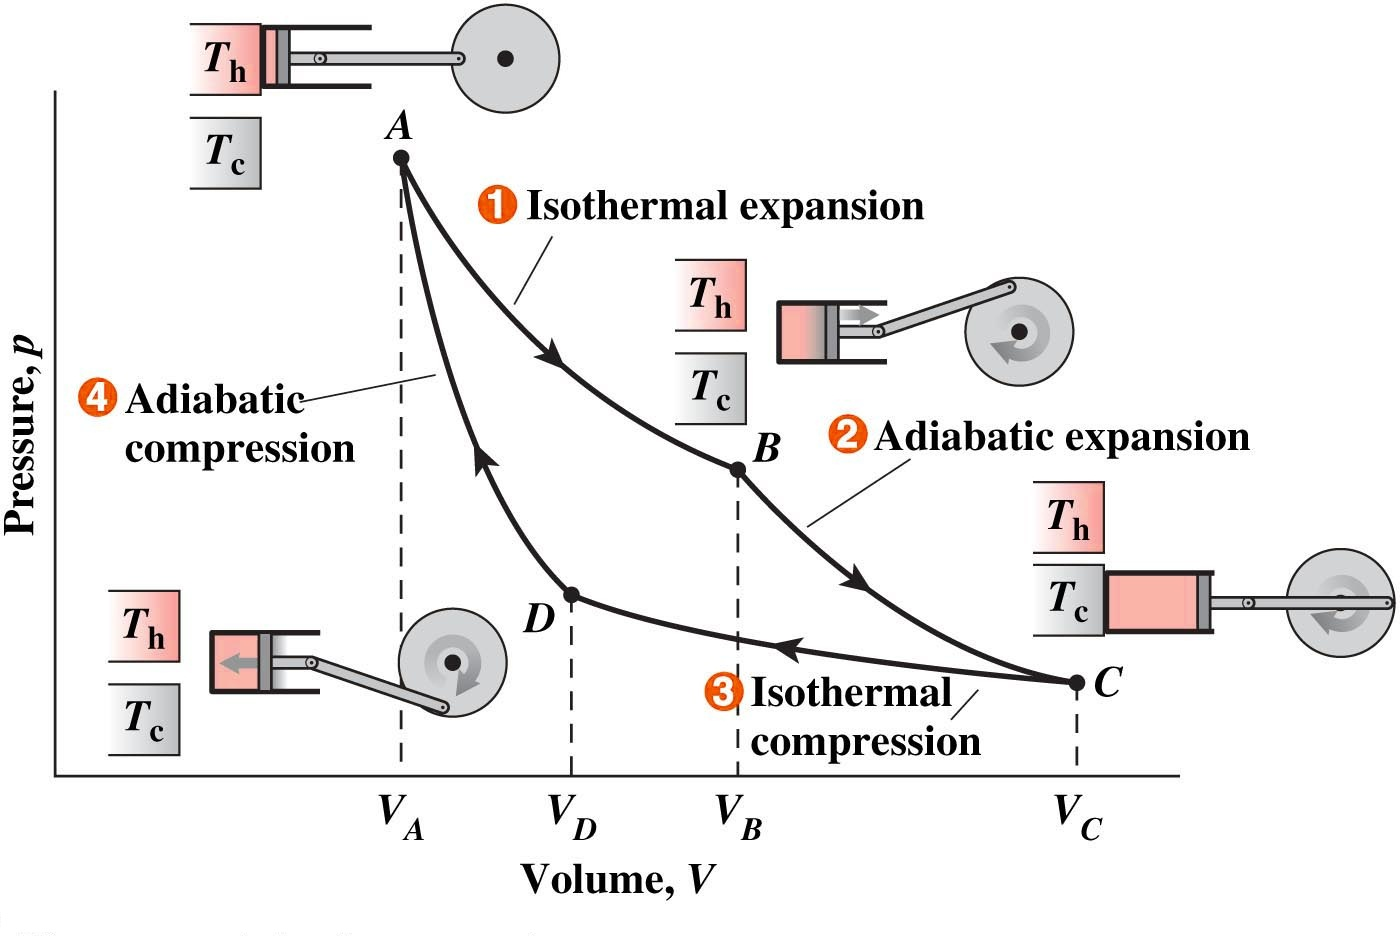
\includegraphics[width=0.8\textwidth]{therm_carnot_fig1}\label{fig:carnotprozess_im_pv_diagramm}
        \caption{\textsc{Carnot}--Prozess im p--V--Diagramm.}
\end{figure}
\begin{figure}
        \centering
        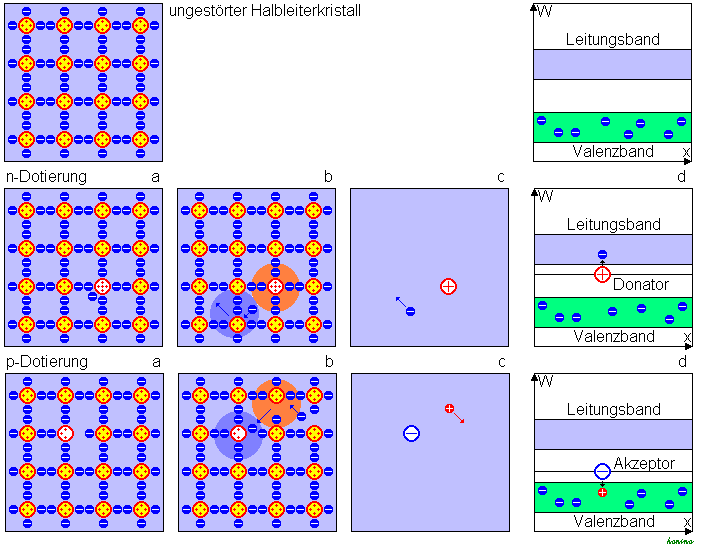
\includegraphics[width=0.7\textwidth]{Halbleiter1}\label{fig:halbleiter}
        \caption{Bändermodell verschiedener Leiter bzw.\ Nichtleiter.}
\end{figure}

%}}}

\end{document}
